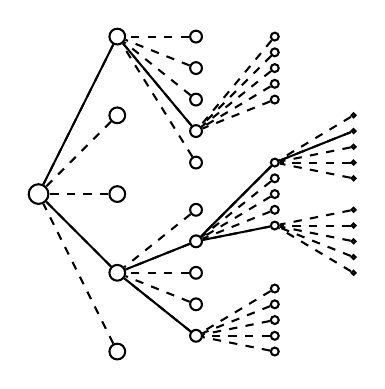
\begin{tikzpicture}
[font=\footnotesize, draw=black, line width=0.75pt,
fragment/.style={circle, draw, inner sep=0pt}]

\node[fragment,minimum size=2.5mm] (x0y0) at (0, 2) {};
\foreach \y in {0, ..., 4} {
    \node[fragment,minimum size=2mm] (x1y\y) at (1, \y) {}
        edge[dashed] (x0y0);
}
\draw (x0y0) -- (x1y4);
\draw (x0y0) -- (x1y1);

\foreach \y/\p in {51/2.4, 52/2.8, 53/3.2,  54/3.6, 55/4.0} {
    \node[fragment,minimum size=1.5mm] (x2y\y) at (2, \p) {}
        edge[dashed] (x1y4);
}
\draw (x1y4) -- (x2y52);

\foreach \y/\p in {21/0.2, 22/0.6, 23/1.0,  24/1.4, 25/1.8} {
    \node[fragment,minimum size=1.5mm] (x2y\y) at (2, \p) {}
        edge[dashed] (x1y1);
}
\draw (x1y1) -- (x2y24);
\draw (x1y1) -- (x2y21);

\foreach \y/\p in {421/3.2, 422/3.4, 423/3.6,  424/3.8, 425/4.0} {
    \node[fragment,minimum size=1mm] (x3y\y) at (3, \p) {}
        edge[dashed] (x2y52);
}

\foreach \y/\p in {241/1.6, 242/1.8, 243/2.0,  244/2.2, 245/2.4} {
    \node[fragment,minimum size=1mm] (x3y\y) at (3, \p) {}
        edge[dashed] (x2y24);
}
\draw (x2y24) -- (x3y241);
\draw (x2y24) -- (x3y245);

\foreach \y/\p in {211/0.0, 212/0.2, 213/0.4,  214/0.6, 215/0.8} {
    \node[fragment,minimum size=1mm] (x3y\y) at (3, \p) {}
        edge[dashed] (x2y21);
}

\foreach \y/\p in {2451/2.2, 2452/2.4, 2453/2.6,  2454/2.8, 2455/3.0} {
    \node[fragment,minimum size=0.5mm] (x4y\y) at (4, \p) {}
        edge[dashed] (x3y245);
}
\draw (x3y245) -- (x4y2454);

\foreach \y/\p in {2411/1.0, 2412/1.2, 2413/1.4,  2414/1.6, 2415/1.8} {
    \node[fragment,minimum size=0.5mm] (x4y\y) at (4, \p) {}
        edge[dashed] (x3y241);
}

\end{tikzpicture}